\chapter{Docker}

\section{Overview}
This chapter documents the installation of Docker on Ubuntu and the successful deployment of two containerized web applications as required for the assignment.

\section{Docker Installation on Ubuntu}
Docker was installed on Ubuntu using the following commands, I had it previously installed so I just verified the installation:

\begin{minted}{bash}
docker --version
docker run hello-world
\end{minted}

\section{First Container: Hello World Web Server}
Created a simple Node.js HTTP server following the assignment instructions. The project structure included \texttt{server.js}, \texttt{package.json}, and \texttt{Dockerfile}.

\subsection{Build and Execution}
\begin{minted}{bash}
docker build -t hello-node .
docker run -p 5050:3000 hello-node
\end{minted}

The application was successfully deployed and accessible at \texttt{http://localhost:5050}.

\begin{figure}[H]
    \centering
    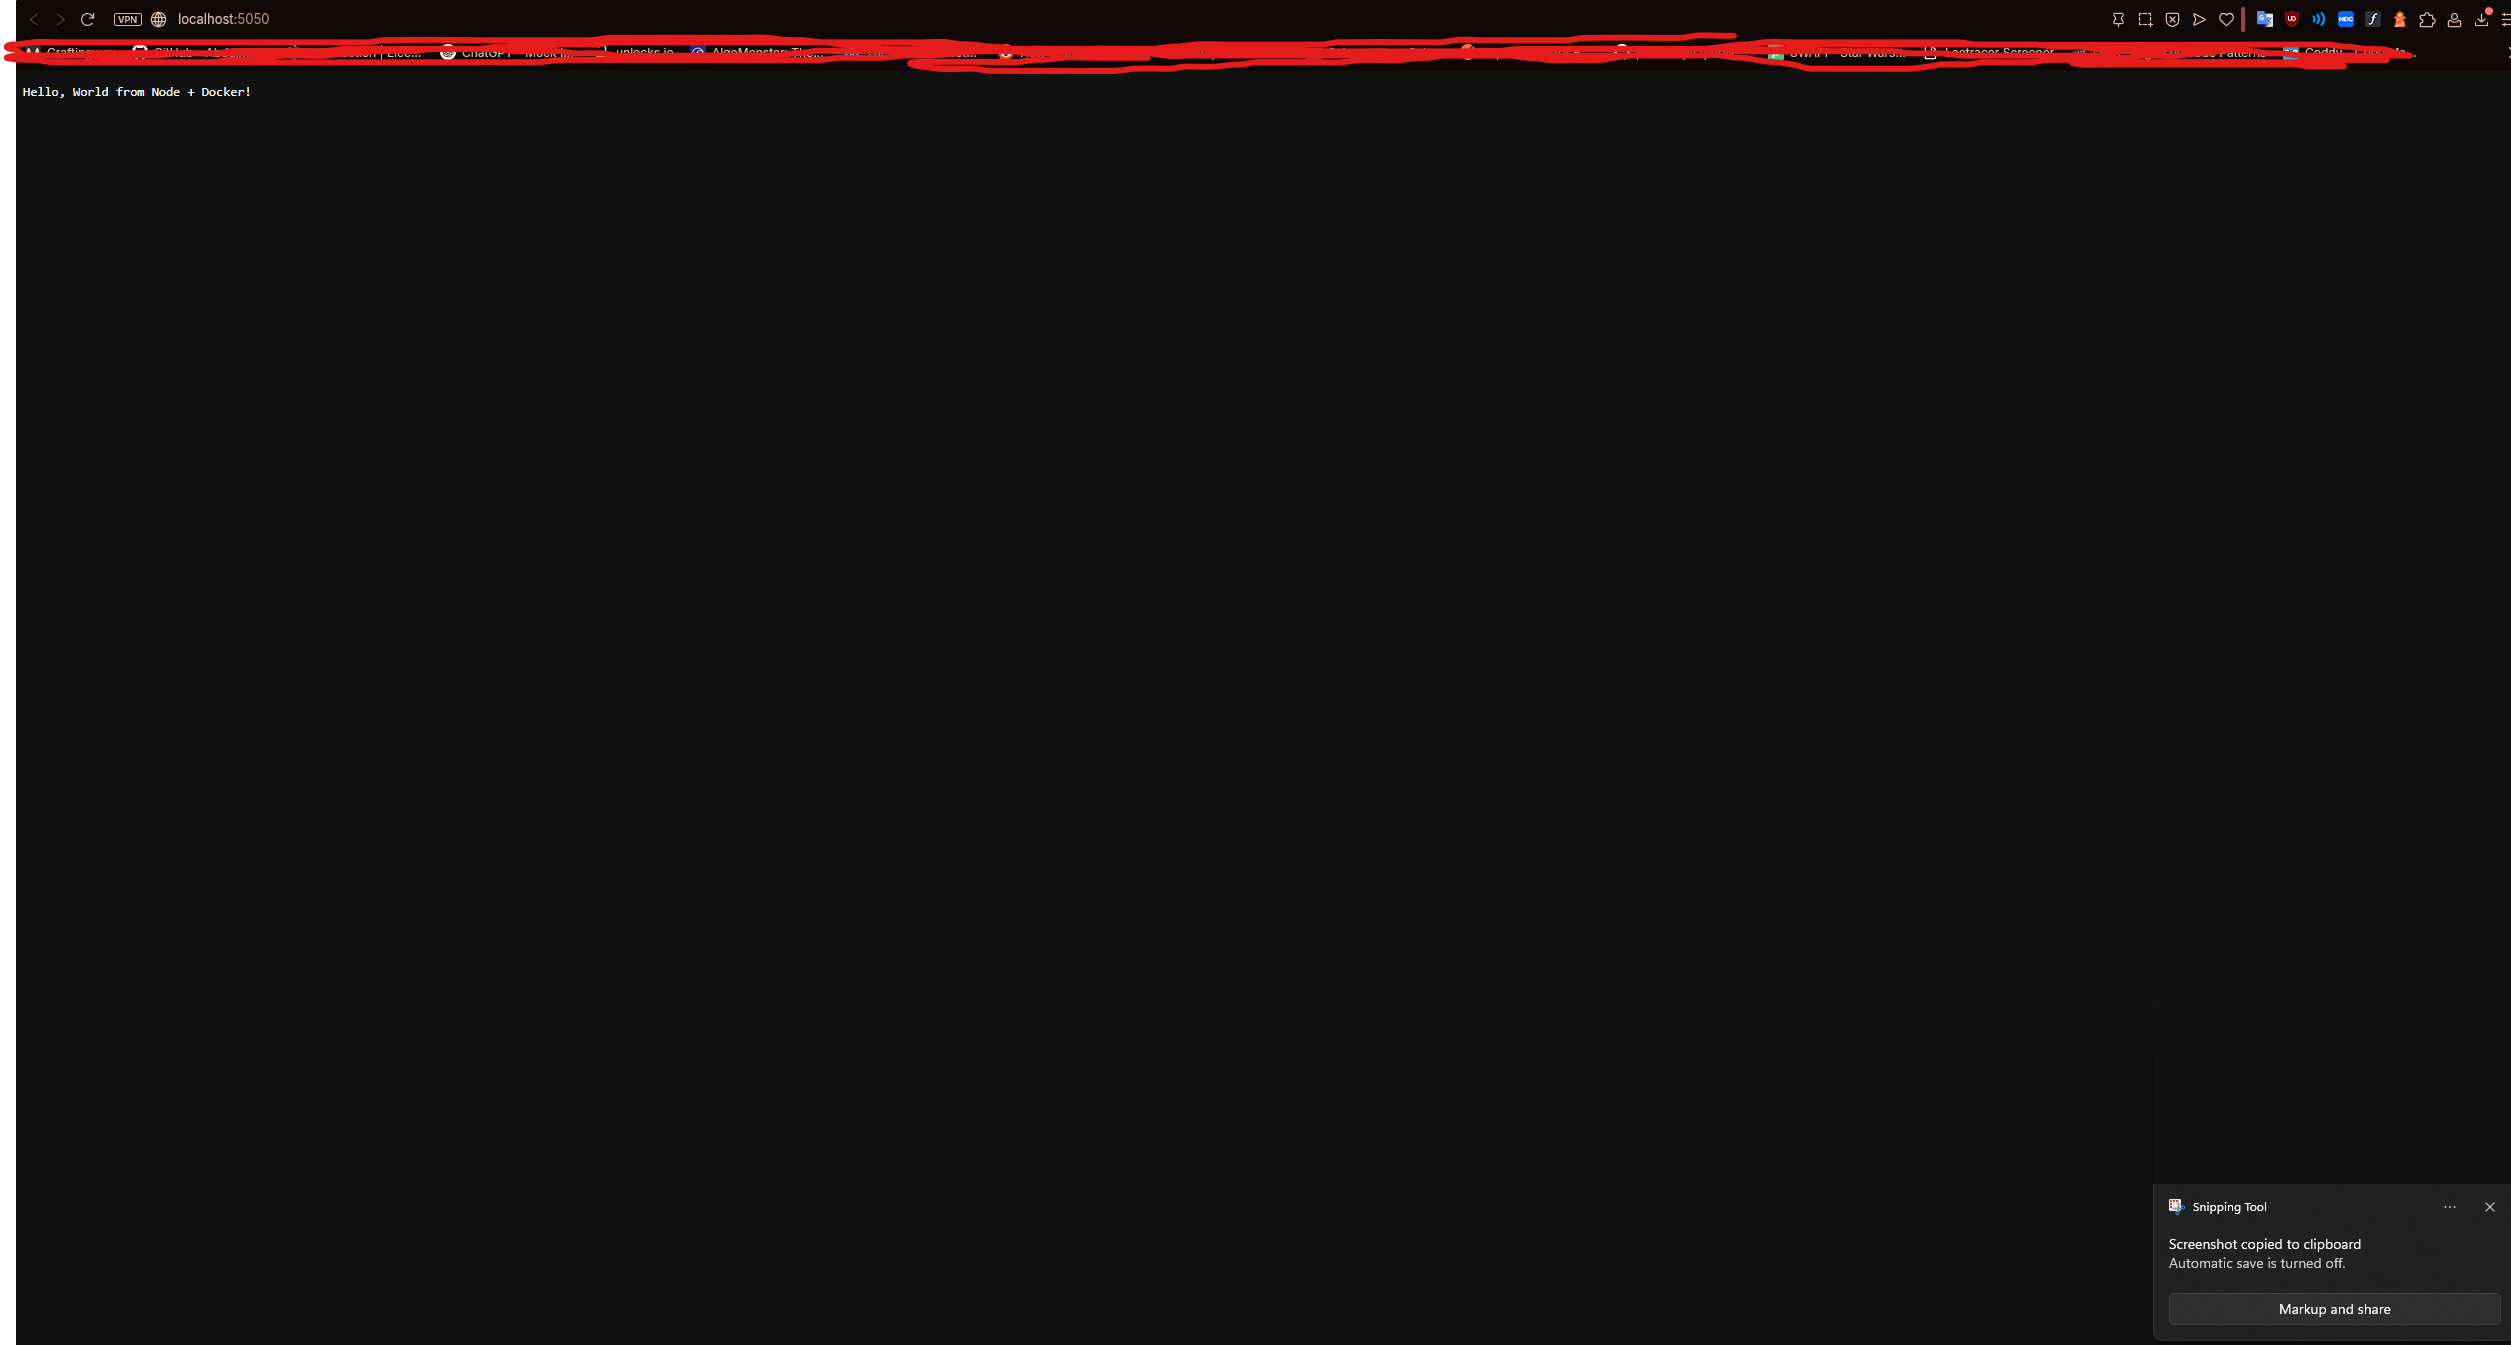
\includegraphics[width=0.8\textwidth]{png/Screenshot 2025-09-23 192048.png}
    \caption{Hello World Node.js application running in Docker container}
    \label{fig:hello-world}
\end{figure}

\section{Second Container: Color Buttons Website}
Created an Express.js web application with interactive color-changing functionality following the assignment specifications.

\subsection{Build and Execution}
\begin{minted}{bash}
docker build -t color-buttons-app .
docker run -p 8080:3000 color-buttons-app
\end{minted}

The application was successfully deployed and accessible at \texttt{http://localhost:8080}.

\begin{figure}[H]
    \centering
    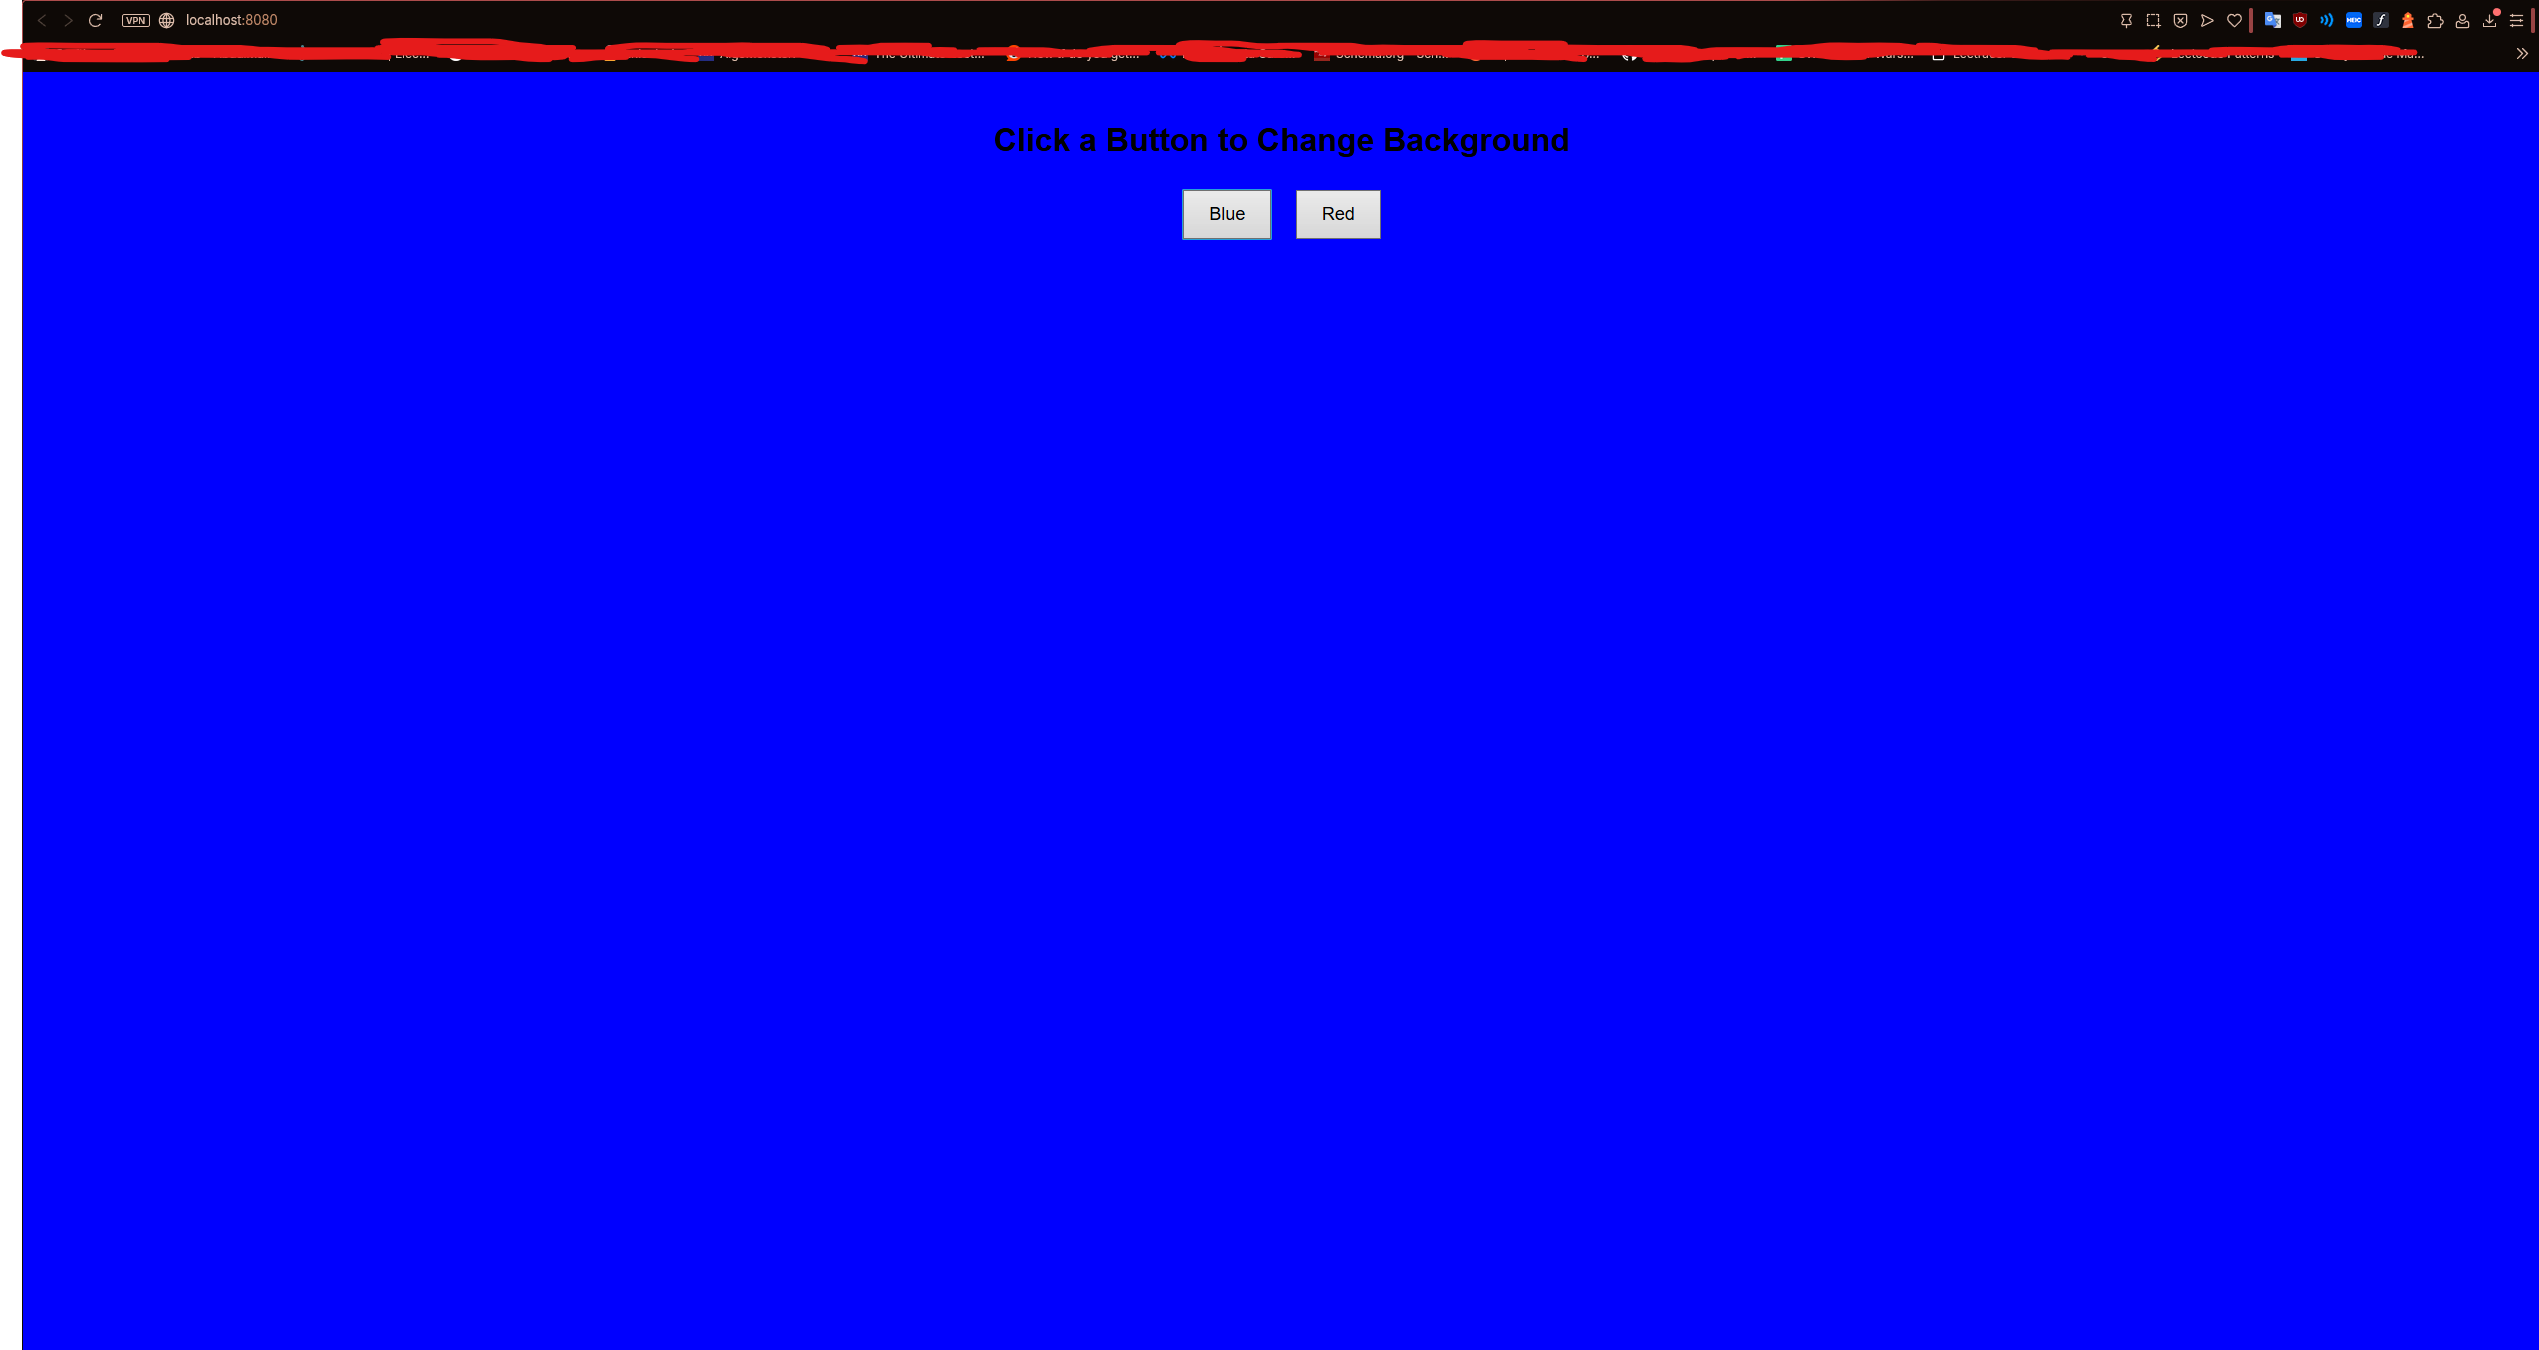
\includegraphics[width=0.8\textwidth]{png/Screenshot 2025-09-23 193125.png}
    \caption{Color Buttons application demonstrating background color change functionality}
    \label{fig:color-buttons}
\end{figure}

\section{Conclusion}
Both Docker containers were successfully created, built, and executed on Ubuntu. The containers ran as expected, serving web content on the mapped ports and demonstrating proper containerization of Node.js applications.